\section{Domænemodel}
\todo[inline]{Thomas M: indsæt diagram og forklar}
\begin{figure}[ht]
\centering
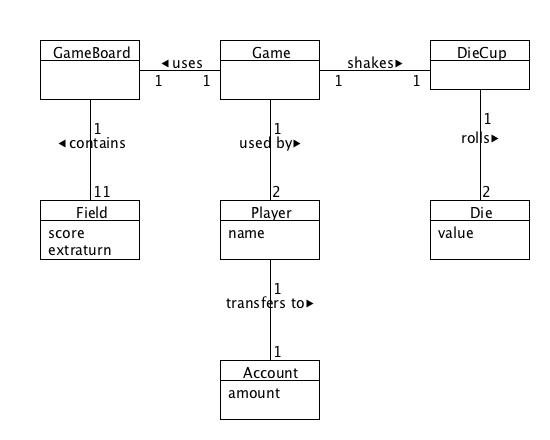
\includegraphics[scale=0.5]{DomainModelDieGame.jpg}
\caption[<Text for the list of figures>]{Domain Model}
\label{fig:figure 2}
\end{figure}
Da vi har kunnet bruge en stor del af vores domænemodel fra sidst, har vi valgt ikke at lave en navneordsanalyse, da vi ville bruge for lang tid på at lave den, i forhold til udbyttet af denne. Dette er årsagen til, at vi starter med domænemodellen.
\\

Vores domæne model er lavet før begyndelse af implementering. Det er udført forinden for at få et overblik over hvilke elementer, vi kunne have behov for i vores program. 
\\


Vi har i diagrammet vist vores hoved domæner. \textit{Game}, som er selve spillet. \textit{Gameboard}, der holder styr på indholdet i spillet. \textit{Field}, som indeholder en score for feltet, og om det giver ekstra tur. \textit{Player}, der bruger spillet. \textit{Account} holder styr på point. \textit{DieCup}, som skal rulle vores terninger. Til sidst har vi \textit{Die} som indeholder terningeværdier, vi skal bruge til at udregne, hvor spilleren lander.